\section{}

\subsection{a) Suitable solutioning temperature and extent of the heat treatment window, and b) primary ageing temperature for new alloy}

\textbf{a)} In figure \ref{fig:diagram05} the amount of all phases is plotted as a function of temperature for the alloy system Ni-Al-Ta-Cr-Re-W-Mo. It shows that the $\gamma'$ curve starts at a composition near $0.8$ value and decreases as the temperature increases, reaching a composition of value $0$ around $1388$°C. The temperature where the composition of the $gamma'$ phase becomes zero is the solutioning temperature. 

The liquid curve corresponds to an approximate temperature of $1380$°C, this temperature corresponds to the solidus temperature, where the liquid phase begins to form. 

The hear treatment window corresponds to de window that exists between the solutioning temperature, $1388$°C, to the solidus temperatures, $1380$°C, which gives a window of approximately $8$°C; so in this range of temperature the $\gamma'$ can be dissolved without partial melting of the alloy.

\begin{figure}[h]
  \centering
    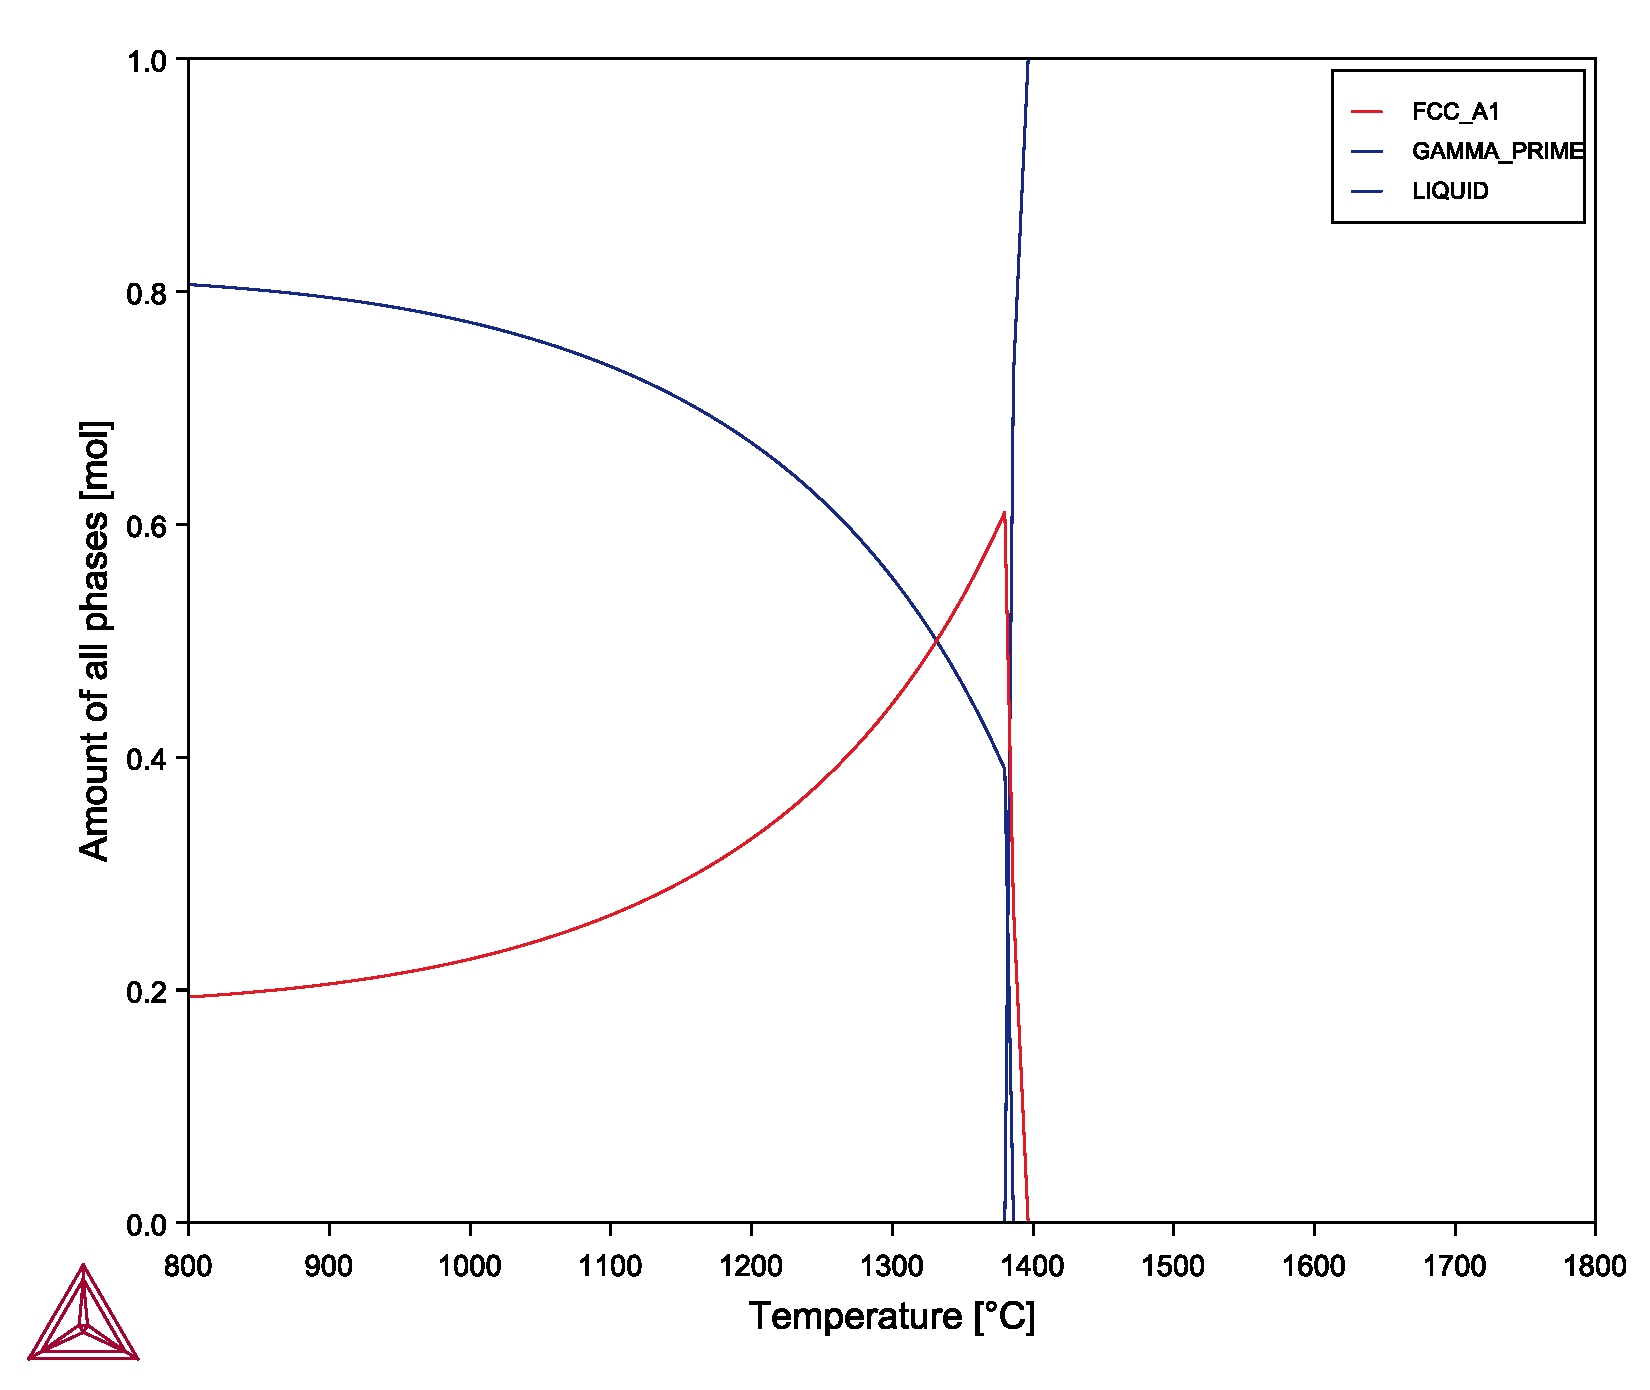
\includegraphics[width=0.95\textwidth]{graficas/Q4_02.pdf}
    \caption{Amount of all phases as a function of temperature generated with \textit{ThermoCalc} \citep{thermocalc}}
    \label{fig:diagram05}
\end{figure}

\textbf{b)} The primary ageing temperature is found at a $\gamma'$ fraction of approximately 0.60, looking at \ref{fig:diagram05} the \shnote{me falta editar la imagen para poder poner ahi el punto donde la curva esta a 0.60}

%The γ′ fraction at lower temperatures is used to define the ageing condition. From the diagram, the γ′ fraction reaches ≈0.60 at a temperature of about 1080 °C. This temperature is therefore selected as the primary ageing temperature, where a stable amount of precipitates can form and strengthen the alloy.

%Why 60% γ′ fraction is used for ageing

%In Ni-based superalloys, the strengthening phase is γ′ (Ni₃Al-type precipitate).

%For good creep resistance and mechanical strength, you want a significant amount of γ′ precipitates but not 100%, because you also need some γ (FCC matrix) for ductility and toughness.

%Experimental alloy design studies have shown that a γ′ volume fraction around 60–70% gives the best balance between strength and workability.